\chapter{RESULTADOS OBTIDOS}
\label{chp:resultadosObtidos}
 
Neste capítulo, serão apresentados os resultados que foram obtidos através da
ferramenta analítica \acs{Google Analytics} e as principais telas do sistema
web proposto por este projeto. Sendo que, os dados estatísticos apresentados
correspondem ao período de 11 de outubro à 09 de novembro de 2014.

Pode-se observar na Figura \ref{fig:googleAnalyticsGrafico}, que a
ferramenta de gestão de perguntas e respostas está sendo acessada quase
que diariamente para gerir as questões postadas na lista de discussão.

\begin{figure}[h!tb]
	\caption{Visualizações de página}
	\label{fig:googleAnalyticsGrafico}

	\centering
	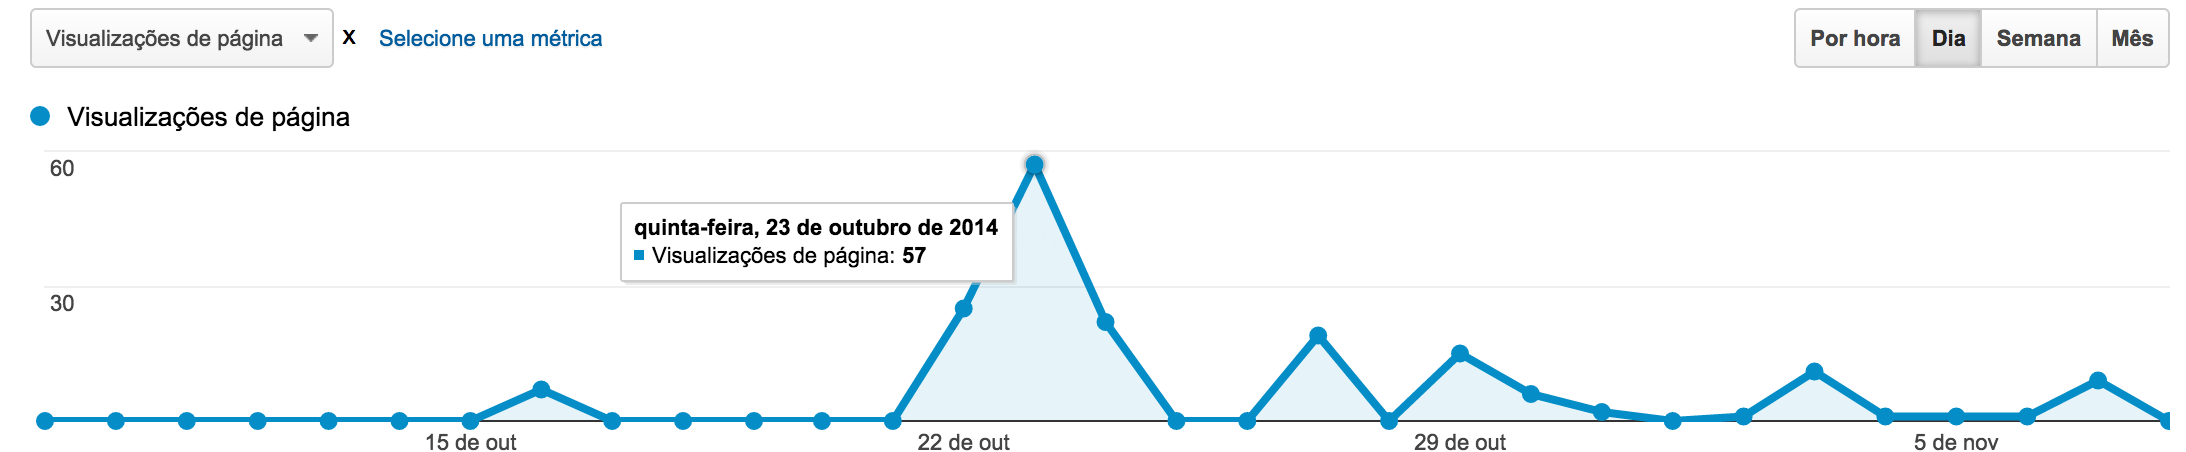
\includegraphics[width=\textwidth]{images/resultados/google-analytics-grafico.png}

	\centering
	\footnotesize Fonte: \fonteOAutor
\end{figure}

\FloatBarrier 	% Este comando impede que as imagens
				% flutuem a partir deste ponto no seu documento

Na data em que a ferramenta foi divulgada ao grupo ``Rumo a certificação PHP''
(no dia 23 de outubro de 2014), conforme exibe-se na Figura
\ref{fig:googleAnalyticsGrafico}, o número de visualizações de página atingiu 
57 \textit{page views}, enquanto que, o autor esperava que o número atingisse
apenas 30 visualizações. Ainda referente a data em que houve a divulgação, 
percebe-se que o tempo de acesso ao sistema também foi bastante elevado, sendo
que o tempo médio para esta única data atingiu 25:04 minutos conforme ilustra a 
Figura \ref{fig:googleAnalyticsTempoAcessoDivulgacao}.

\begin{figure}[h!tb]
	\caption{Tempo de acesso ao sistema no dia da divulgação da ferramenta}
	\label{fig:googleAnalyticsTempoAcessoDivulgacao}

	\centering
	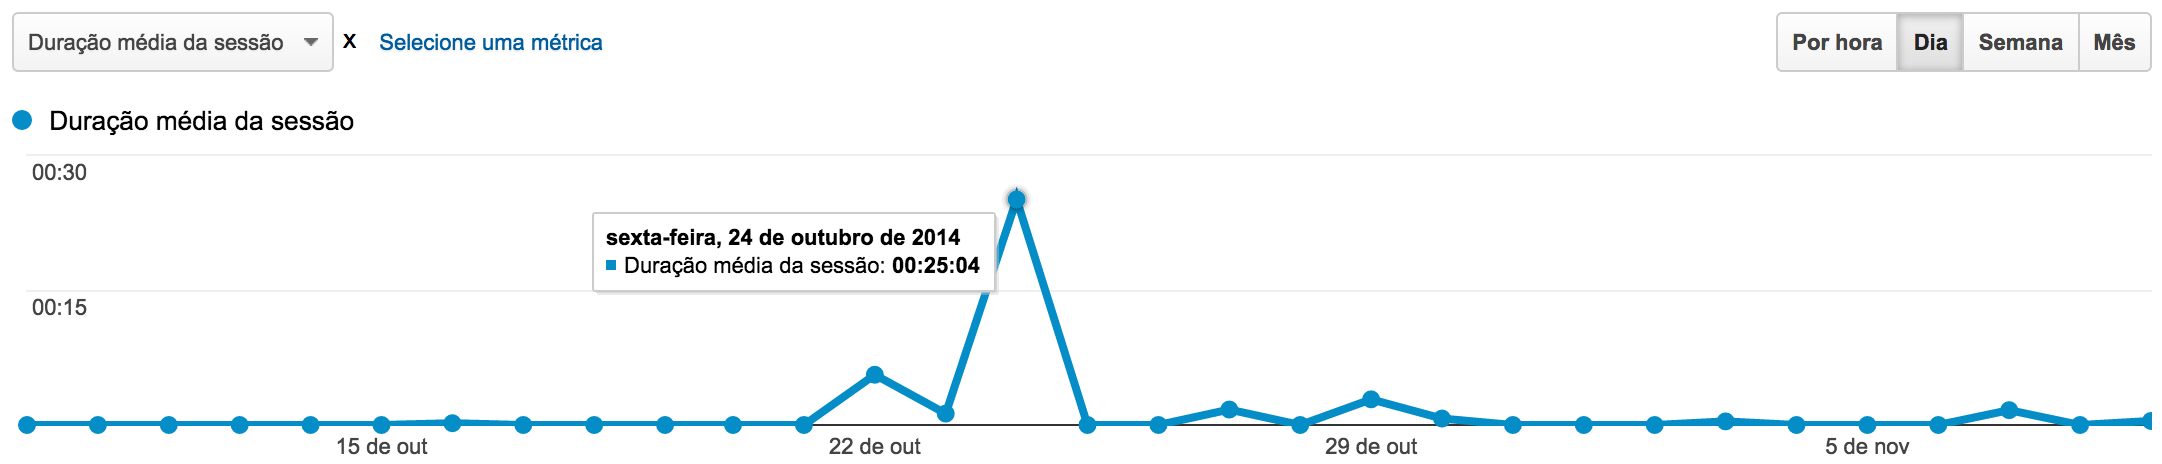
\includegraphics[width=\textwidth]{images/resultados/google-analytics-tempoacesso-divulgacao.png}

	\centering
	\footnotesize Fonte: \fonteOAutor
\end{figure}

\FloatBarrier 	% Este comando impede que as imagens
				% flutuem a partir deste ponto no seu documento
				
Nota-se também que nos dias seguintes a quantidade de visualizações de página
se estabilizou, onde removendo a data de divulgação da contagem a fim de não
influenciar no resultado final da média, foi obtido o valor de 25,40 acessos
semanais conforme os dados apresentados na Figura \ref{fig:googleAnalyticsMediaVisualizacoes}.

\begin{figure}[h!tb]
	\caption{Quantidade de visualizações de página semanais}
	\label{fig:googleAnalyticsMediaVisualizacoes}

	\centering
	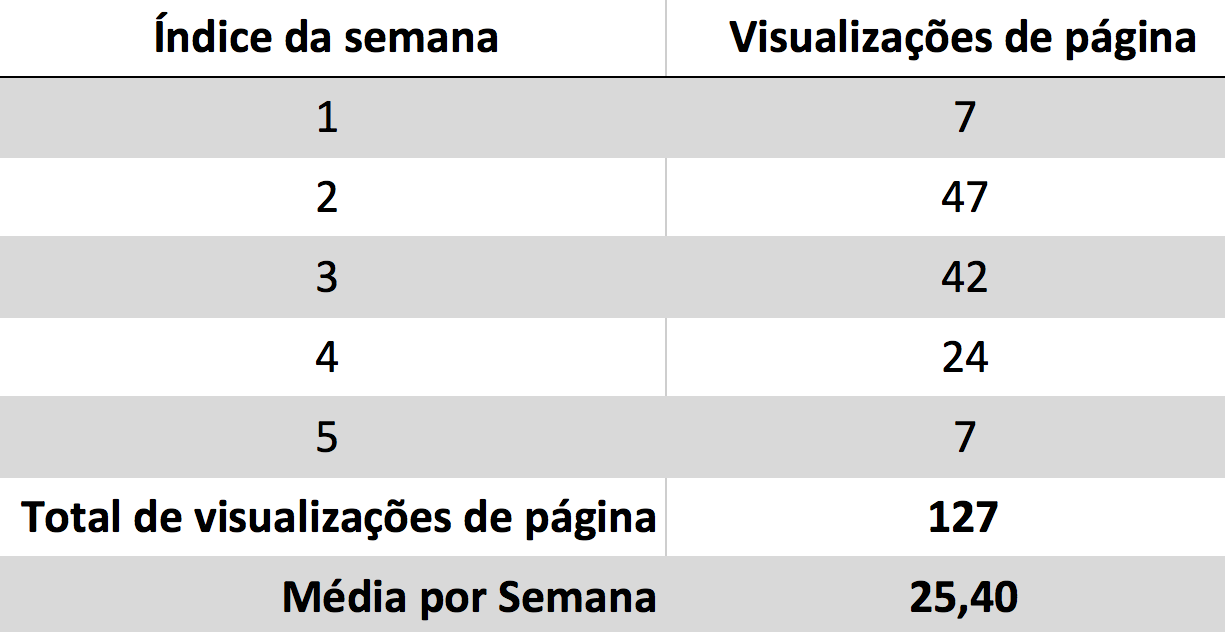
\includegraphics[width=0.6\textwidth]{images/resultados/google-analytics-media-visualizacoes.png}

	\centering
	\footnotesize Fonte: \fonteOAutor
\end{figure}

\FloatBarrier 	% Este comando impede que as imagens
				% flutuem a partir deste ponto no seu documento

Na Figura \ref{fig:googleAnalyticsCidade}, exibe-se as cidades que deram
origem aos acessos à ferramenta de gestão de perguntas e respostas, sendo
que, dentre elas está a cidade de Joinville/SC que é a cidade do autor.

\begin{figure}[h!tb]
	\caption{Cidades em que o acesso ao sistema foi realizado}
	\label{fig:googleAnalyticsCidade}

	\centering
	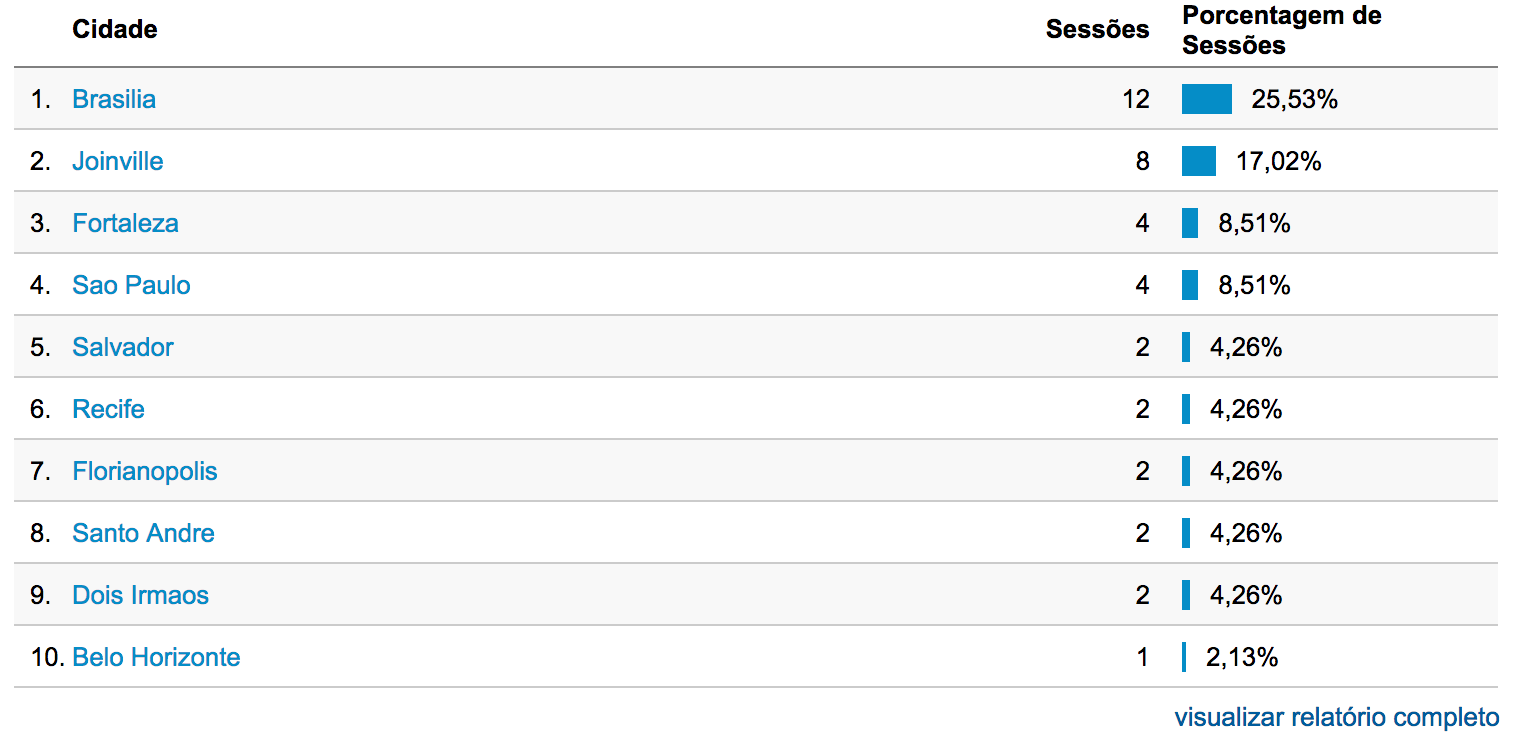
\includegraphics[width=\textwidth]{images/resultados/google-analytics-cidade.png}

	\centering
	\footnotesize Fonte: \fonteOAutor
\end{figure}

\FloatBarrier 	% Este comando impede que as imagens
				% flutuem a partir deste ponto no seu documento
			
Referente a estatísticas de formas de acesso, nenhum uso de \textit{smartphone}
ou \textit{tablet} foi registrado, mas nota-se que dentre os sistemas
operacionais dos profissionais que utilizaram a aplicação está o
\textit{Windows} com 46,81\%, o \textit{Macintosh} com 29,79\% e o
\textit{Linux} com 23,40\%, e em contrapartida, o navegador web mais utilizado 
para o uso da ferramenta foi o \textit{Google Chrome} com 57,45\% do total,
seguido pelo \textit{Firefox} com 38,30\% e pelo \textit{Safari} com 4,26\%
conforme apresenta-se na Figura
\ref{fig:googleAnalyticsSistemaOperacionalNavegador}.

\begin{figure}[h!tb]
	\caption{Sistemas Operacionais e Navegadores utilizados para acesso ao
	sistema web}
	\label{fig:googleAnalyticsSistemaOperacionalNavegador}

	\centering
	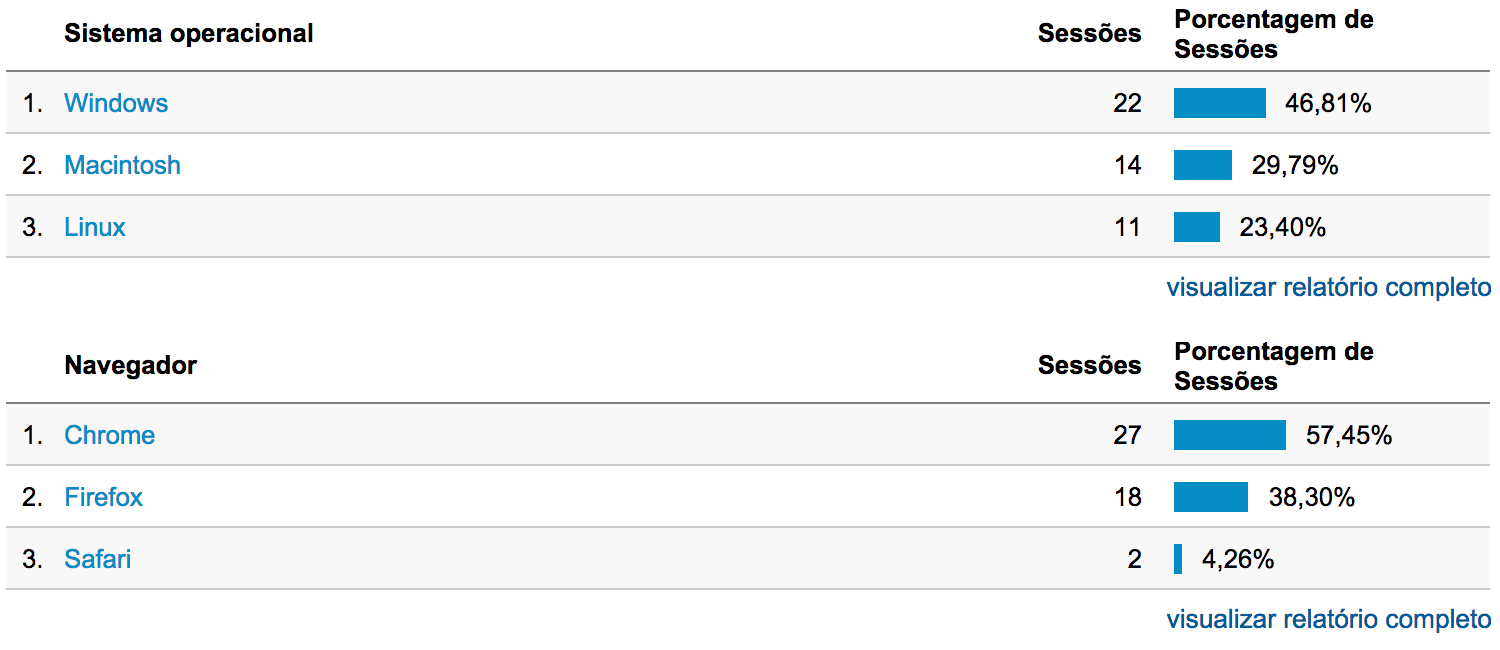
\includegraphics[width=\textwidth]{images/resultados/google-analytics-os-browser.png}

	\centering
	\footnotesize Fonte: \fonteOAutor
\end{figure}

\FloatBarrier 	% Este comando impede que as imagens
				% flutuem a partir deste ponto no seu documento

Nota-se ainda, conforme ilustra a Figura \ref{fig:googleAnalyticsTempoAcesso},
que o tempo médio de acesso à ferramenta é de 02:01 minutos o que permite que um 
colaborador da lista de discussão acesse o sistema gere uma pergunta diária de
maneira anonima e em seguida encerre a sessão, justificando também a taxa de
rejeição de 31,91\%.

\begin{figure}[h!tb]
	\caption{Tempo médio de permanência de um usuário na ferramenta}
	\label{fig:googleAnalyticsTempoAcesso}

	\centering
	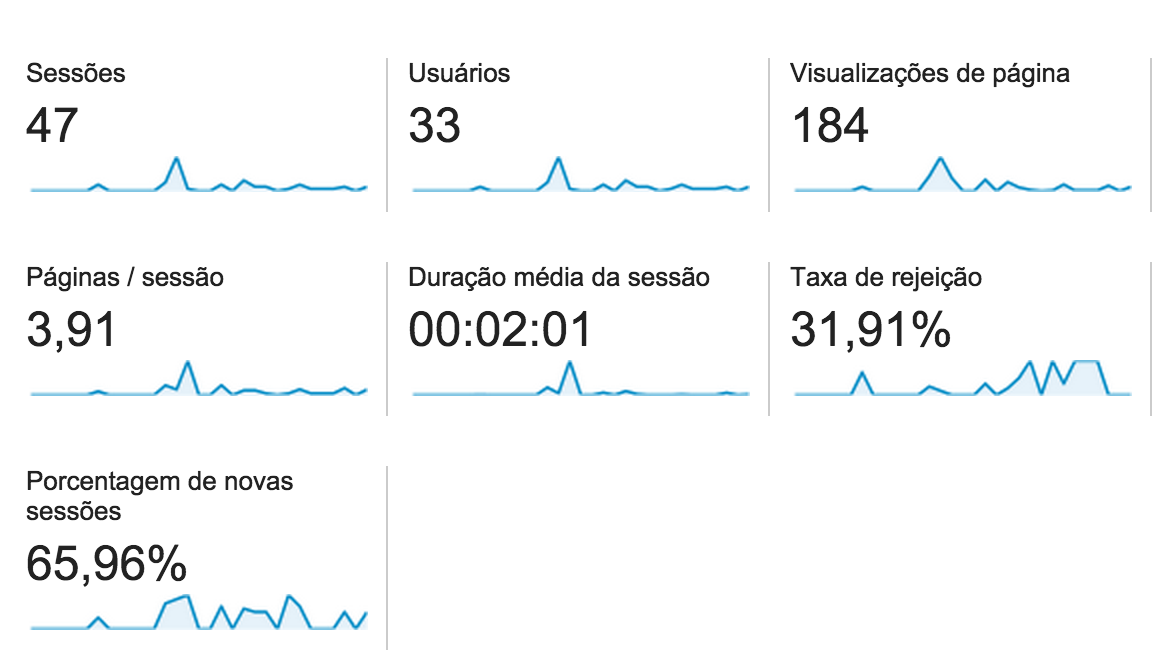
\includegraphics[width=0.7\textwidth]{images/resultados/google-analytics-dados.png}

	\centering
	\footnotesize Fonte: \fonteOAutor
\end{figure}

\FloatBarrier 	% Este comando impede que as imagens
				% flutuem a partir deste ponto no seu documento

Além disto, percebe-se na Figura \ref{fig:googleAnalyticsTempoAcesso} que dentre
as 47 sessões existentes, os 33 usuários navegaram pelo sistema acessando quase
quatro páginas por sessão, outro detalhe importante, é que houve na média mais
do que um acesso por dia ao sistema o que fortalece o fato de que a ferramenta
está sendo utilizada para gerir as perguntas diárias postadas na lista de
discussão.

Na Figura \ref{fig:googleAnalyticsPaginas}, exibe-se as páginas mais acessadas
da aplicação web, nota-se que, todos os usuários entram na página inicial e em
seguida a maioria acessa de forma anonima, entretanto alguns antes de efetuarem
tal ação selecionam um idioma (dentre os disponíveis estão o português do
brasil e o inglês internacional).

\begin{figure}[h!tb]
	\caption{Páginas do sistema mais acessadas}
	\label{fig:googleAnalyticsPaginas}

	\centering
	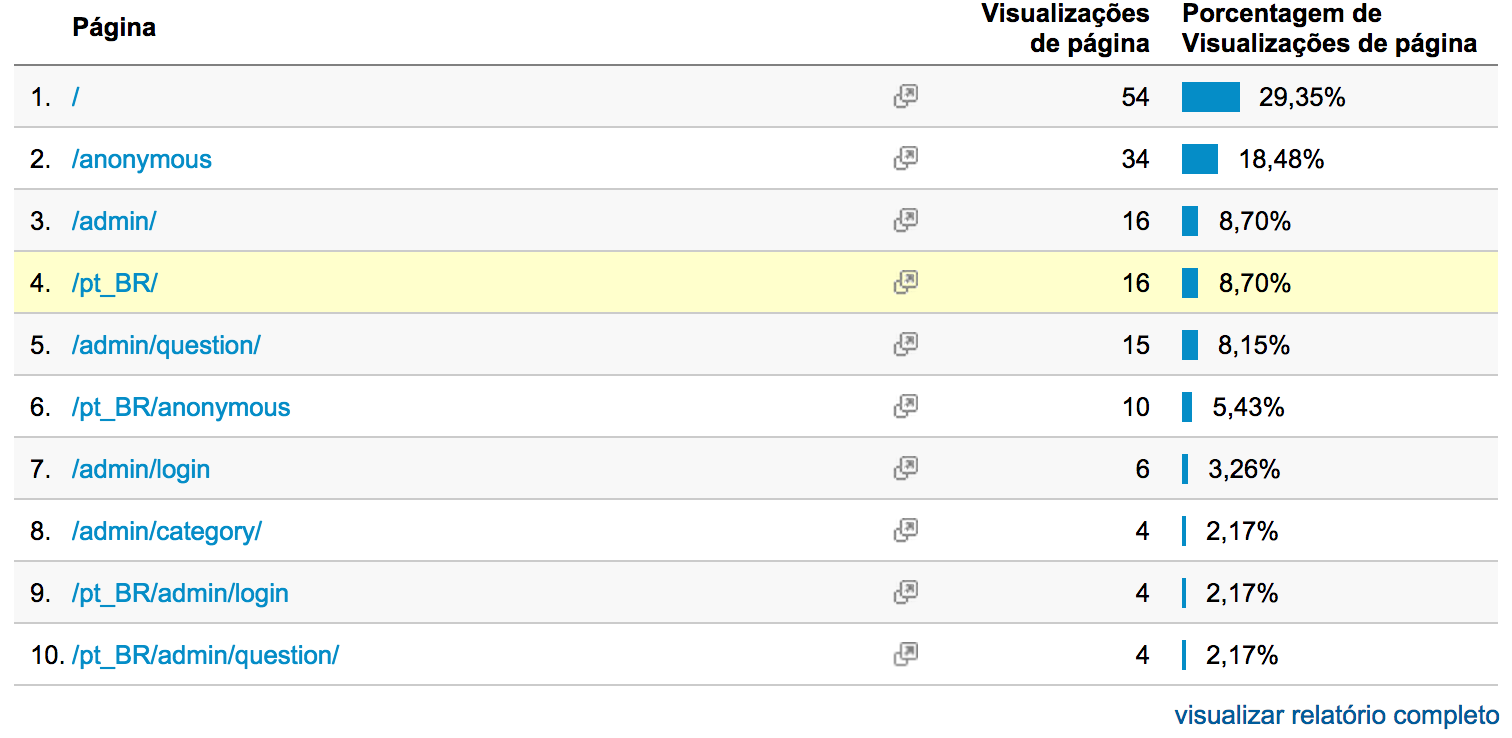
\includegraphics[width=\textwidth]{images/resultados/google-analytics-paginas.png}

	\centering
	\footnotesize Fonte: \fonteOAutor
\end{figure}

\FloatBarrier 	% Este comando impede que as imagens
				% flutuem a partir deste ponto no seu documento

No que diz respeito ao idioma de acesso do sistema, na Figura
\ref{fig:googleAnalyticsIdioma}, exibe-se a quantidade de acessos categorizados
através do idioma dos usuários.

\begin{figure}[h!tb]
	\caption{Idioma dos usuários que realizaram acesso à ferramenta}
	\label{fig:googleAnalyticsIdioma}

	\centering
	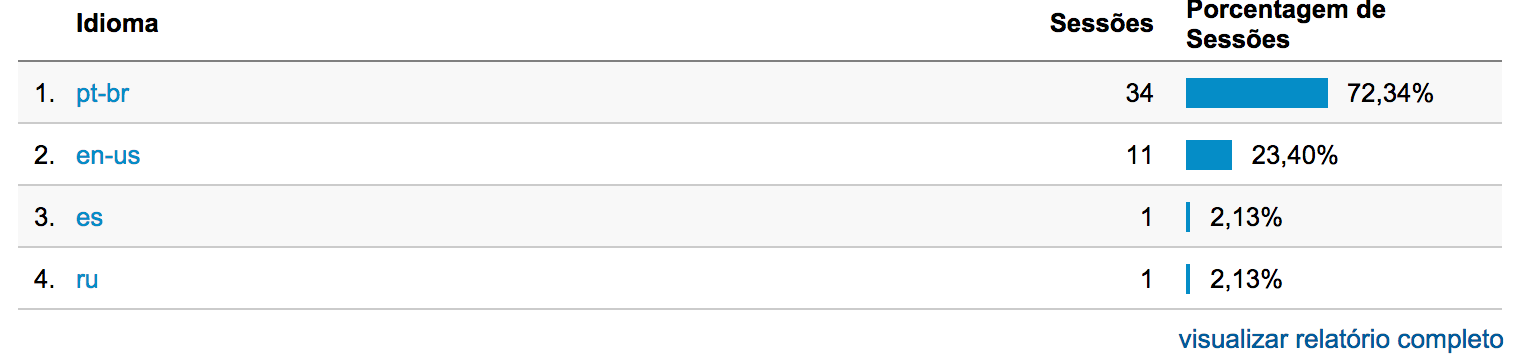
\includegraphics[width=\textwidth]{images/resultados/google-analytics-idioma.png}

	\centering
	\footnotesize Fonte: \fonteOAutor
\end{figure}

\FloatBarrier 	% Este comando impede que as imagens
				% flutuem a partir deste ponto no seu documento




% Agora as imagens do sistema

Na Figura XX, exibe-se a página inicial do sistema que apresenta três maneiras
de uso da plataforma.. 

IMAGEM DA TELA INICIAL DO SISTEMA

FALAR SOBRE AS 3 FORMAS DE USO

FALAR SOBRE OS NÍVEIS DE ACESSO DO SISTEMA (GRUPOS DE USUÁRIOS)

Nota-se também que o sistema proposto está internacionalizado e já conta com
dois idiomas, o português do Brasil e o inglês internacional conforme mostra a
Figura XX.

IMAGEM DA TELA INICIAL DO SISTEMA EM INGLÊS

A listagem de perguntas apresentada na Figura XX, é o resultado da categorizacao
de perguntas e respostas da lista de discussão, sendo que, nesta listagem
apresentam-se dados básicos para o usuário que está logado, e para os usuários
administradores algumas informacoes adicionais sao exibidas: são elas.. XX e XX

IMAGEM DA LISTAGEM DE PERGUNTAS E RESPOSTAS

A Figura XX, mostra-se a exibicão dos tópicos da lista de discussão diretamente
do \textit{Google Groups}, onde evidencia-se que não há somente o banco de dados
de perguntas e respostas, mas também assuntos referente a outros temas que na
Figura XX, é o caso do ``Acesso ao Dropbox''.

FALAR TAMBÉM PELA FACILIDADE DE BUSCAR UMA QUESTÃO E SABER A QUANTIDADE DE
QUESTÕES CADASTRADAS

IMAGEM DA LISTAGEM DE PERGUNTAS E RESPOSTAS DO GOOGLE GROUPS

Neste momento apresenta-se em detalhes na Figura XX, a representacão da exibicão
de detalhes de uma questão que está sendo gerenciada através da ferramenta
proposta.

IMAGEM DE DETALHES DE UMA QUESTÃO DA FERRAMENTA

Nota-se também que todas as informacões que o sistema mantém referente a questão
são exibidos, sendo que, as linhas XX e XX são exibidas somente para os usuários
com permissões administrativas.

A seguir apresenta-se na Figura XX, a mesma questão na plataforma do
\textit{Google Groups} no qual não há nenhum gerenciamento das questões que
foram postadas, diferentemente da nova forma de gestão de perguntas proposta por
este projeto.

IMAGEM DE DETALHES DE UMA QUESTÃO DA FERRAMENTA DO GOOGLE GROUPS

Como já havia sido citado, a ferramenta está sendo utilizada e está disponível
no seguinte endereco: \textit{http://zcpe.cekurte.com}.
